\documentclass[,man,floatsintext]{apa6}
\usepackage{lmodern}
\usepackage{amssymb,amsmath}
\usepackage{ifxetex,ifluatex}
\usepackage{fixltx2e} % provides \textsubscript
\ifnum 0\ifxetex 1\fi\ifluatex 1\fi=0 % if pdftex
  \usepackage[T1]{fontenc}
  \usepackage[utf8]{inputenc}
\else % if luatex or xelatex
  \ifxetex
    \usepackage{mathspec}
  \else
    \usepackage{fontspec}
  \fi
  \defaultfontfeatures{Ligatures=TeX,Scale=MatchLowercase}
\fi
% use upquote if available, for straight quotes in verbatim environments
\IfFileExists{upquote.sty}{\usepackage{upquote}}{}
% use microtype if available
\IfFileExists{microtype.sty}{%
\usepackage{microtype}
\UseMicrotypeSet[protrusion]{basicmath} % disable protrusion for tt fonts
}{}
\usepackage{hyperref}
\hypersetup{unicode=true,
            pdftitle={Supplementary Materials: Early language experience in a Papuan village},
            pdfauthor={Marisa Casillas, Penelope Brown, \& Stephen C. Levinson},
            pdfborder={0 0 0},
            breaklinks=true}
\urlstyle{same}  % don't use monospace font for urls
\usepackage{graphicx}
% grffile has become a legacy package: https://ctan.org/pkg/grffile
\IfFileExists{grffile.sty}{%
\usepackage{grffile}
}{}
\makeatletter
\def\maxwidth{\ifdim\Gin@nat@width>\linewidth\linewidth\else\Gin@nat@width\fi}
\def\maxheight{\ifdim\Gin@nat@height>\textheight\textheight\else\Gin@nat@height\fi}
\makeatother
% Scale images if necessary, so that they will not overflow the page
% margins by default, and it is still possible to overwrite the defaults
% using explicit options in \includegraphics[width, height, ...]{}
\setkeys{Gin}{width=\maxwidth,height=\maxheight,keepaspectratio}
\IfFileExists{parskip.sty}{%
\usepackage{parskip}
}{% else
\setlength{\parindent}{0pt}
\setlength{\parskip}{6pt plus 2pt minus 1pt}
}
\setlength{\emergencystretch}{3em}  % prevent overfull lines
\providecommand{\tightlist}{%
  \setlength{\itemsep}{0pt}\setlength{\parskip}{0pt}}
\setcounter{secnumdepth}{0}
% Redefines (sub)paragraphs to behave more like sections
\ifx\paragraph\undefined\else
\let\oldparagraph\paragraph
\renewcommand{\paragraph}[1]{\oldparagraph{#1}\mbox{}}
\fi
\ifx\subparagraph\undefined\else
\let\oldsubparagraph\subparagraph
\renewcommand{\subparagraph}[1]{\oldsubparagraph{#1}\mbox{}}
\fi

%%% Use protect on footnotes to avoid problems with footnotes in titles
\let\rmarkdownfootnote\footnote%
\def\footnote{\protect\rmarkdownfootnote}


  \title{Supplementary Materials: Early language experience in a Papuan village}
    \author{Marisa Casillas\textsuperscript{1}, Penelope Brown\textsuperscript{1},
\& Stephen C. Levinson\textsuperscript{1}}
    \date{}
  
\shorttitle{Supp. Materials: Early language experience in a Papuan village}
\affiliation{
\vspace{0.5cm}
\textsuperscript{1} Max Planck Institute for Psycholinguistics}
\usepackage{csquotes}
\usepackage{upgreek}
\captionsetup{font=singlespacing,justification=justified}

\usepackage{longtable}
\usepackage{lscape}
\usepackage{multirow}
\usepackage{tabularx}
\usepackage[flushleft]{threeparttable}
\usepackage{threeparttablex}

\newenvironment{lltable}{\begin{landscape}\begin{center}\begin{ThreePartTable}}{\end{ThreePartTable}\end{center}\end{landscape}}

\makeatletter
\newcommand\LastLTentrywidth{1em}
\newlength\longtablewidth
\setlength{\longtablewidth}{1in}
\newcommand{\getlongtablewidth}{\begingroup \ifcsname LT@\roman{LT@tables}\endcsname \global\longtablewidth=0pt \renewcommand{\LT@entry}[2]{\global\advance\longtablewidth by ##2\relax\gdef\LastLTentrywidth{##2}}\@nameuse{LT@\roman{LT@tables}} \fi \endgroup}


\usepackage{lineno}

\linenumbers
\usepackage{float}
\floatplacement{figure}{H}
\usepackage{placeins}

\authornote{

Correspondence concerning this article should be addressed to Marisa
Casillas, P.O. Box 310, 6500 AH Nijmegen, The Netherlands. E-mail:
\href{mailto:Marisa.Casillas@mpi.nl}{\nolinkurl{Marisa.Casillas@mpi.nl}}}

\abstract{

}

\begin{document}
\maketitle

\section{Full model outputs}\label{models}

In these Supplementary Materials we give the full model output tables
for each analysis in the main text, including re-leveled versions of
each model to show all three of the two-way contrasts between the
three-level time-of-day factor (i.e., morning vs.~midday, morning
vs.~afternoon, and midday vs.~afternoon) as well as, for each of the
measures, a histogram showing how each variable is distributed (i.e.,
because they are non-normal and/or zero-inflated) and a figure showing
the distribution of model residuals. For every negative binomial model,
we also include the full model output table and residual plots for
matching gaussian mixed-effects regressions which use a log-transformed
dependent measure. Such gaussian models with log-transformed measures
are an alternative solution to analyzing non-normal distributions
sometimes used in psycholinguistics, but are not suitable for the
current data given how our speech environment measures are distributed,
particularly in the randomly sampled clips (see, e.g., Figures
\protect\hyperlink{fig1}{1}, \protect\hyperlink{fig7}{7},
\protect\hyperlink{fig10}{10}, \protect\hyperlink{fig13}{13},
\protect\hyperlink{fig19}{19}). Overall, the gaussian models show a
qualitatively similar pattern of results. These analyses are structured
as identically as possible to those in Casillas and colleagues'
(forthcoming) study on Tseltal Mayan child language environments.

\subsection{How to interpret the model
output}\label{how-to-interpret-the-model-output}

All models were run with the glmm-TMB library in R (Brooks et al.,
2017a, 2017b). Note that, in the negative binomial regressions, the
dependent variables have been rounded to the nearest integer (e.g., 3.2
minutes of TCDS per hour becomes 3 minutes per hour in the model).

The predictors in the models are abbreviated as follows: tchiyr.std =
centered, standardized target child age in months; stthr.tri = the start
time of the clip as either morning, midday, or afternoon; hsz.std =
centered, standardized household size of the target child; nsk.std =
centered, standardized number of speakers present in the clip,
aclew\_child\_id = the unique identifier for each child. The predictors
are sometimes combined in two-way interactions, as shown below with a
\enquote{:} separator between predictor names (e.g., tchiyr.std:nsk.std
= a two-way interaction of target child age and number of speakers
present).

In each model output table, the \enquote{component} shows what kind of
model the estimate derives from (e.g., the zero-inflated models include
both a conditional \enquote{cond} set of predictors, random effects, and
zero-inflation \enquote{zi} predictors). The \enquote{term} is the
estimated predictor. The \enquote{statistic} is the estimated
\emph{z}-statistic for each predictor's effect. The other labels are
self-explanatory.

As more data are added to this corpus, the analyses will also be
updated, as will this supplementary model information, all of which will
be available online at:
\url{https://middycasillas.shinyapps.io/Yeli_Child_Language_Environment/}.

\subsection{Target-child-directed speech (TCDS)}\label{models-tcds}

\subsubsection{Random clips}\label{models-tcds-random}

TCDS rate in the random clips demonstrated a skewed distribution with
extra cases of zero (\protect\hyperlink{fig1}{Figure 1}). We therefore
modeled it using a zero-inflated negative binomial mixed-effects
regression in the main text: results for the two models demonstrating
all pairwise effects of time of day are shown in
\protect\hyperlink{tab1}{Table 1} and \protect\hyperlink{tab2}{Table 2}.
The residuals for the default model (\protect\hyperlink{tab1}{Table 1})
are shown in \protect\hyperlink{fig2}{Figure 2}.

\FloatBarrier

\begin{figure}[H]

{\centering 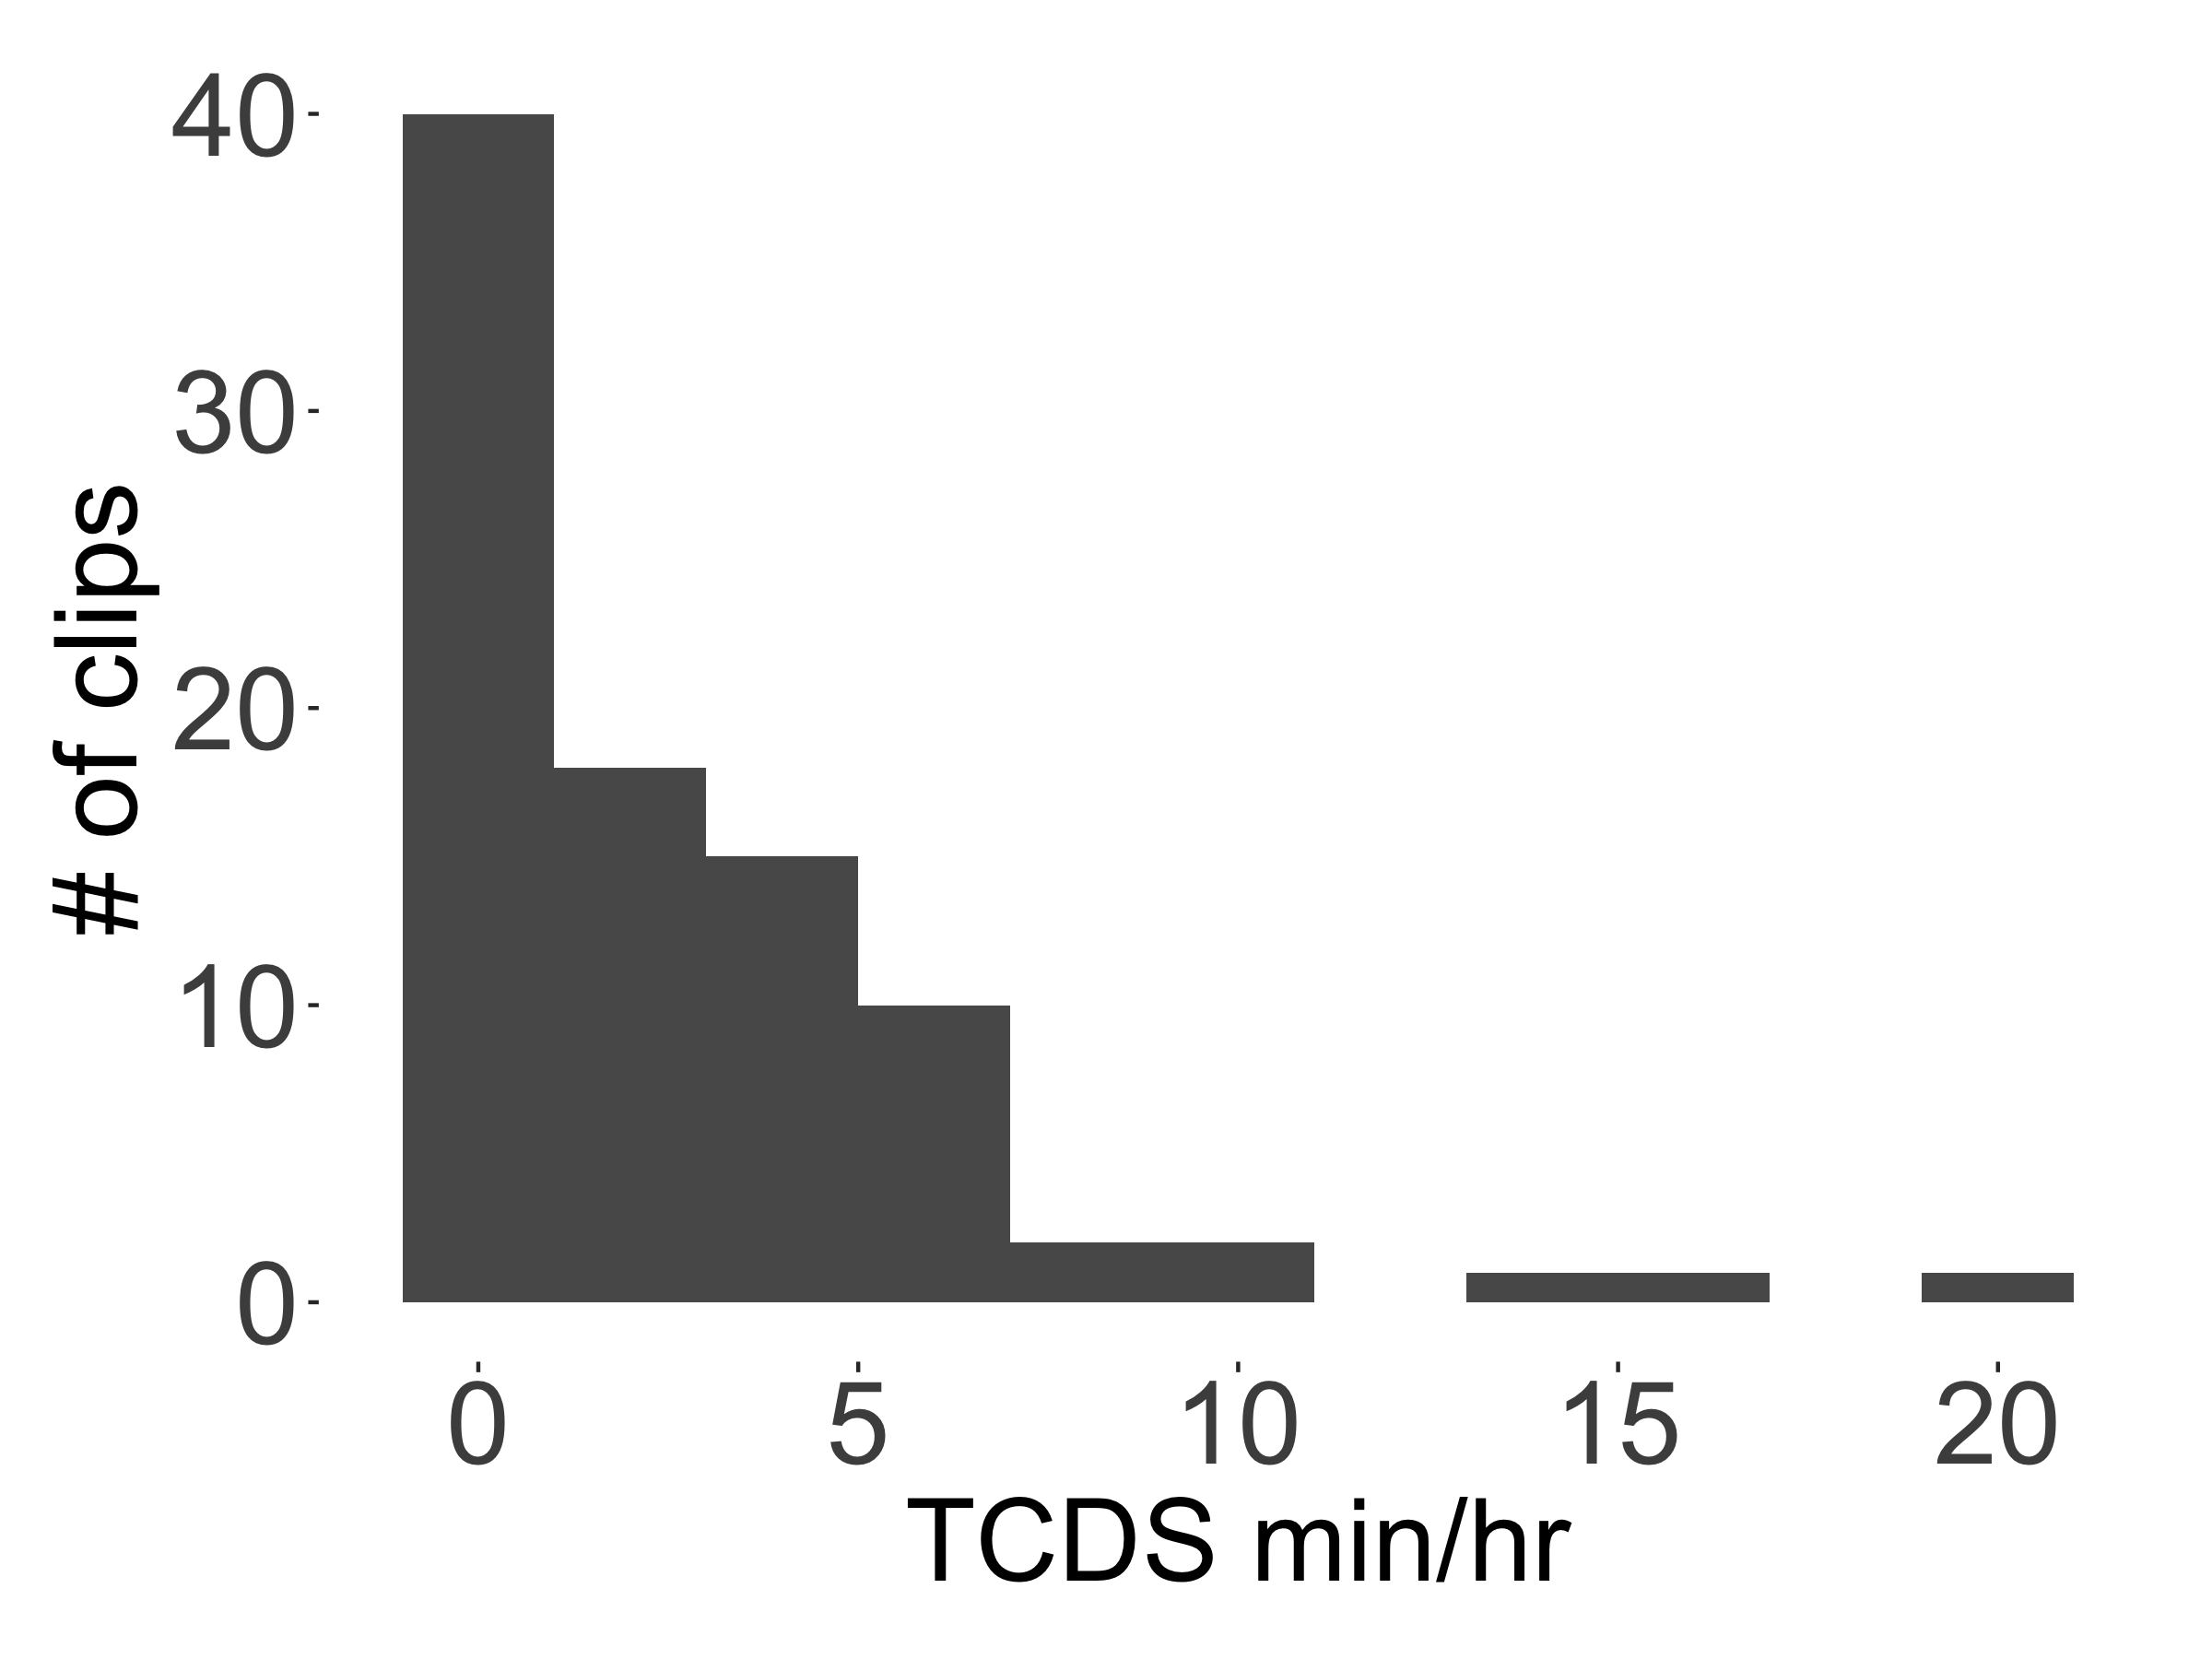
\includegraphics[width=0.4\linewidth]{www/TCDS_random_distribution} 

}

\caption{The distribution of TCDS rates found across the 90 random clips.}\label{fig:fig1}
\end{figure}

\FloatBarrier

\begin{table}[tbp]
\begin{center}
\begin{threeparttable}
\caption{\label{tab:tab1}Full output of the zero-inflated negative binomial mixed-effects regression of TCDS min/hr for the random sample, with midday as the reference level for time of day.}
\begin{tabular}{llllll}
\toprule
component & \multicolumn{1}{c}{term} & \multicolumn{1}{c}{estimate} & \multicolumn{1}{c}{std.error} & \multicolumn{1}{c}{statistic} & \multicolumn{1}{c}{p.value}\\
\midrule
cond & (Intercept) & 0.69 & 0.32 & 2.16 & 0.03\\
cond & tchiyr.std & 0.73 & 0.23 & 3.20 & 0.00\\
cond & stthr.trimorning & 0.80 & 0.36 & 2.23 & 0.03\\
cond & stthr.triafternoon & 0.26 & 0.35 & 0.73 & 0.46\\
cond & hsz.std & -0.21 & 0.12 & -1.69 & 0.09\\
cond & nsk.std & -0.04 & 0.16 & -0.27 & 0.79\\
cond & tchiyr.std:stthr.trimorning & -0.59 & 0.30 & -1.94 & 0.05\\
cond & tchiyr.std:stthr.triafternoon & -0.60 & 0.29 & -2.04 & 0.04\\
cond & tchiyr.std:nsk.std & -0.03 & 0.11 & -0.26 & 0.80\\
zi & (Intercept) & -9.28 & 11.51 & -0.81 & 0.42\\
zi & nsk.std & -5.66 & 7.44 & -0.76 & 0.45\\
random\_effect & aclew\_child\_id & 0.00 & NA & NA & NA\\
\bottomrule
\end{tabular}
\end{threeparttable}
\end{center}
\end{table}

\begin{table}[tbp]
\begin{center}
\begin{threeparttable}
\caption{\label{tab:tab2}Full output of the zero-inflated negative binomial mixed-effects regression of TCDS min/hr for the random sample, with afternoon as the reference level for time of day.}
\begin{tabular}{llllll}
\toprule
component & \multicolumn{1}{c}{term} & \multicolumn{1}{c}{estimate} & \multicolumn{1}{c}{std.error} & \multicolumn{1}{c}{statistic} & \multicolumn{1}{c}{p.value}\\
\midrule
cond & (Intercept) & 0.95 & 0.19 & 4.99 & 0.00\\
cond & tchiyr.std & 0.14 & 0.19 & 0.72 & 0.47\\
cond & stthr.tri.amidday & -0.26 & 0.35 & -0.73 & 0.46\\
cond & stthr.tri.amorning & 0.54 & 0.26 & 2.10 & 0.04\\
cond & hsz.std & -0.21 & 0.12 & -1.69 & 0.09\\
cond & nsk.std & -0.04 & 0.16 & -0.27 & 0.79\\
cond & tchiyr.std:stthr.tri.amidday & 0.60 & 0.29 & 2.04 & 0.04\\
cond & tchiyr.std:stthr.tri.amorning & 0.01 & 0.27 & 0.03 & 0.98\\
cond & tchiyr.std:nsk.std & -0.03 & 0.11 & -0.26 & 0.80\\
zi & (Intercept) & -9.28 & 11.51 & -0.81 & 0.42\\
zi & nsk.std & -5.66 & 7.44 & -0.76 & 0.45\\
random\_effect & aclew\_child\_id & 0.00 & NA & NA & NA\\
\bottomrule
\end{tabular}
\end{threeparttable}
\end{center}
\end{table}

\FloatBarrier

\begin{figure}[H]

{\centering 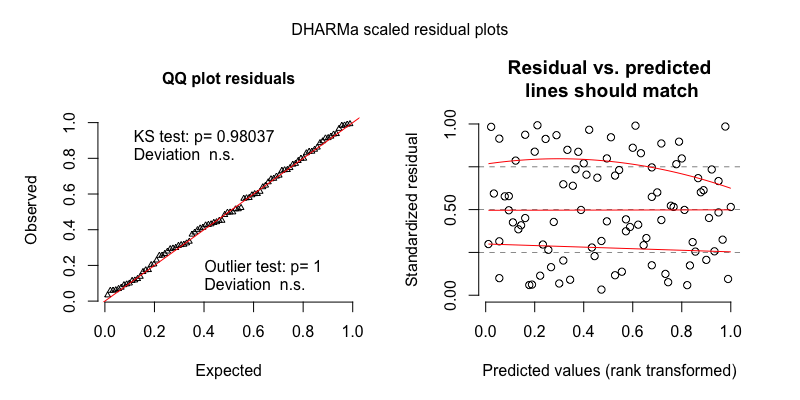
\includegraphics[width=0.9\linewidth]{www/TCDS_random_z-inb_res_plot} 

}

\caption{The model residuals from the zero-inflated negative binomial mixed-effects regression of TCDS min/hr for the random sample.}\label{fig:fig2}
\end{figure}

As an alternative analysis we generated parallel models of TCDS rate in
the random clips using gaussian mixed-effects regression with logged
values of TCDS: results for the two models demonstrating all pairwise
effects of time of day are shown in \protect\hyperlink{tab3}{Table 3}
and \protect\hyperlink{tab4}{Table 4}. The residuals for the default
gaussian model (\protect\hyperlink{tab3}{Table 3}) are shown in
\protect\hyperlink{fig3}{Figure 3}.

\FloatBarrier

\begin{table}[tbp]
\begin{center}
\begin{threeparttable}
\caption{\label{tab:tab3}Full output of the gaussian mixed-effects regression of TCDS min/hr for the random sample, with midday as the reference level for time of day.}
\begin{tabular}{llllll}
\toprule
component & \multicolumn{1}{c}{term} & \multicolumn{1}{c}{estimate} & \multicolumn{1}{c}{std.error} & \multicolumn{1}{c}{statistic} & \multicolumn{1}{c}{p.value}\\
\midrule
cond & (Intercept) & 0.89 & 0.18 & 5.04 & 0.00\\
cond & tchiyr.std & 0.48 & 0.17 & 2.80 & 0.00\\
cond & stthr.trimorning & 0.40 & 0.24 & 1.68 & 0.09\\
cond & stthr.triafternoon & 0.09 & 0.21 & 0.42 & 0.67\\
cond & hsz.std & -0.11 & 0.09 & -1.26 & 0.21\\
cond & nsk.std & 0.03 & 0.09 & 0.35 & 0.73\\
cond & tchiyr.std:stthr.trimorning & -0.39 & 0.25 & -1.56 & 0.12\\
cond & tchiyr.std:stthr.triafternoon & -0.41 & 0.22 & -1.88 & 0.06\\
cond & tchiyr.std:nsk.std & -0.03 & 0.08 & -0.33 & 0.74\\
random\_effect & aclew\_child\_id & 0.00 & NA & NA & NA\\
random\_effect & Residual & 0.79 & NA & NA & NA\\
\bottomrule
\end{tabular}
\end{threeparttable}
\end{center}
\end{table}

\begin{table}[tbp]
\begin{center}
\begin{threeparttable}
\caption{\label{tab:tab4}Full output of the gaussian mixed-effects regression of TCDS min/hr for the random sample, with afternoon as the reference level for time of day.}
\begin{tabular}{llllll}
\toprule
component & \multicolumn{1}{c}{term} & \multicolumn{1}{c}{estimate} & \multicolumn{1}{c}{std.error} & \multicolumn{1}{c}{statistic} & \multicolumn{1}{c}{p.value}\\
\midrule
cond & (Intercept) & 0.98 & 0.12 & 8.11 & 0.00\\
cond & tchiyr.std & 0.08 & 0.13 & 0.58 & 0.56\\
cond & stthr.tri.amidday & -0.09 & 0.21 & -0.42 & 0.67\\
cond & stthr.tri.amorning & 0.31 & 0.20 & 1.56 & 0.12\\
cond & hsz.std & -0.11 & 0.09 & -1.26 & 0.21\\
cond & nsk.std & 0.03 & 0.09 & 0.35 & 0.73\\
cond & tchiyr.std:stthr.tri.amidday & 0.41 & 0.22 & 1.88 & 0.06\\
cond & tchiyr.std:stthr.tri.amorning & 0.02 & 0.22 & 0.10 & 0.92\\
cond & tchiyr.std:nsk.std & -0.03 & 0.08 & -0.33 & 0.74\\
random\_effect & aclew\_child\_id & 0.00 & NA & NA & NA\\
random\_effect & Residual & 0.79 & NA & NA & NA\\
\bottomrule
\end{tabular}
\end{threeparttable}
\end{center}
\end{table}

\FloatBarrier

\begin{figure}[H]

{\centering 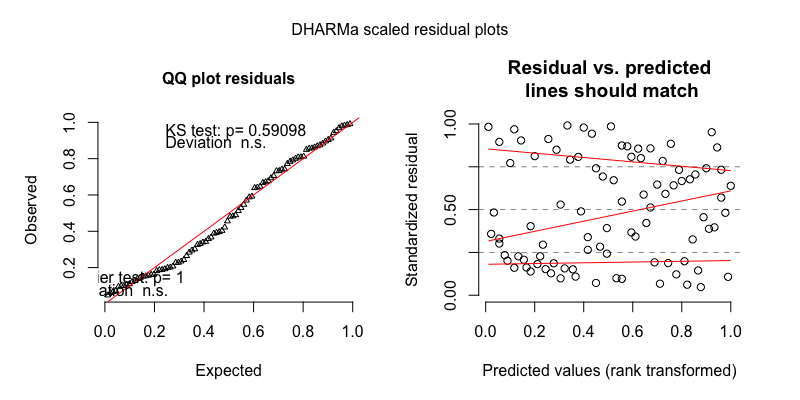
\includegraphics[width=0.9\linewidth]{www/TCDS_random_log_gaus_res_plot} 

}

\caption{The model residuals from the gaussian mixed-effects regression of TCDS min/hr for the random sample.}\label{fig:fig3}
\end{figure}

\FloatBarrier

\subsubsection{Turn-taking clips}\label{models-tcds-turntaking}

TCDS rate in the turn-taking clips demonstrated a slightly skewed, but
unimodal distribution \protect\hyperlink{fig4}{Figure 4}. We therefore
modeled it using a plain (i.e., non-zero-inflated) negative binomial
mixed-effects regression in the main text: results for the two models
demonstrating all pairwise effects of time of day are shown in
\protect\hyperlink{tab5}{Table 5} and \protect\hyperlink{tab6}{Table 6}.
The residuals for the default model (\protect\hyperlink{tab5}{Table 5})
are shown in \protect\hyperlink{fig5}{Figure 5}.

\FloatBarrier

\begin{figure}[H]

{\centering 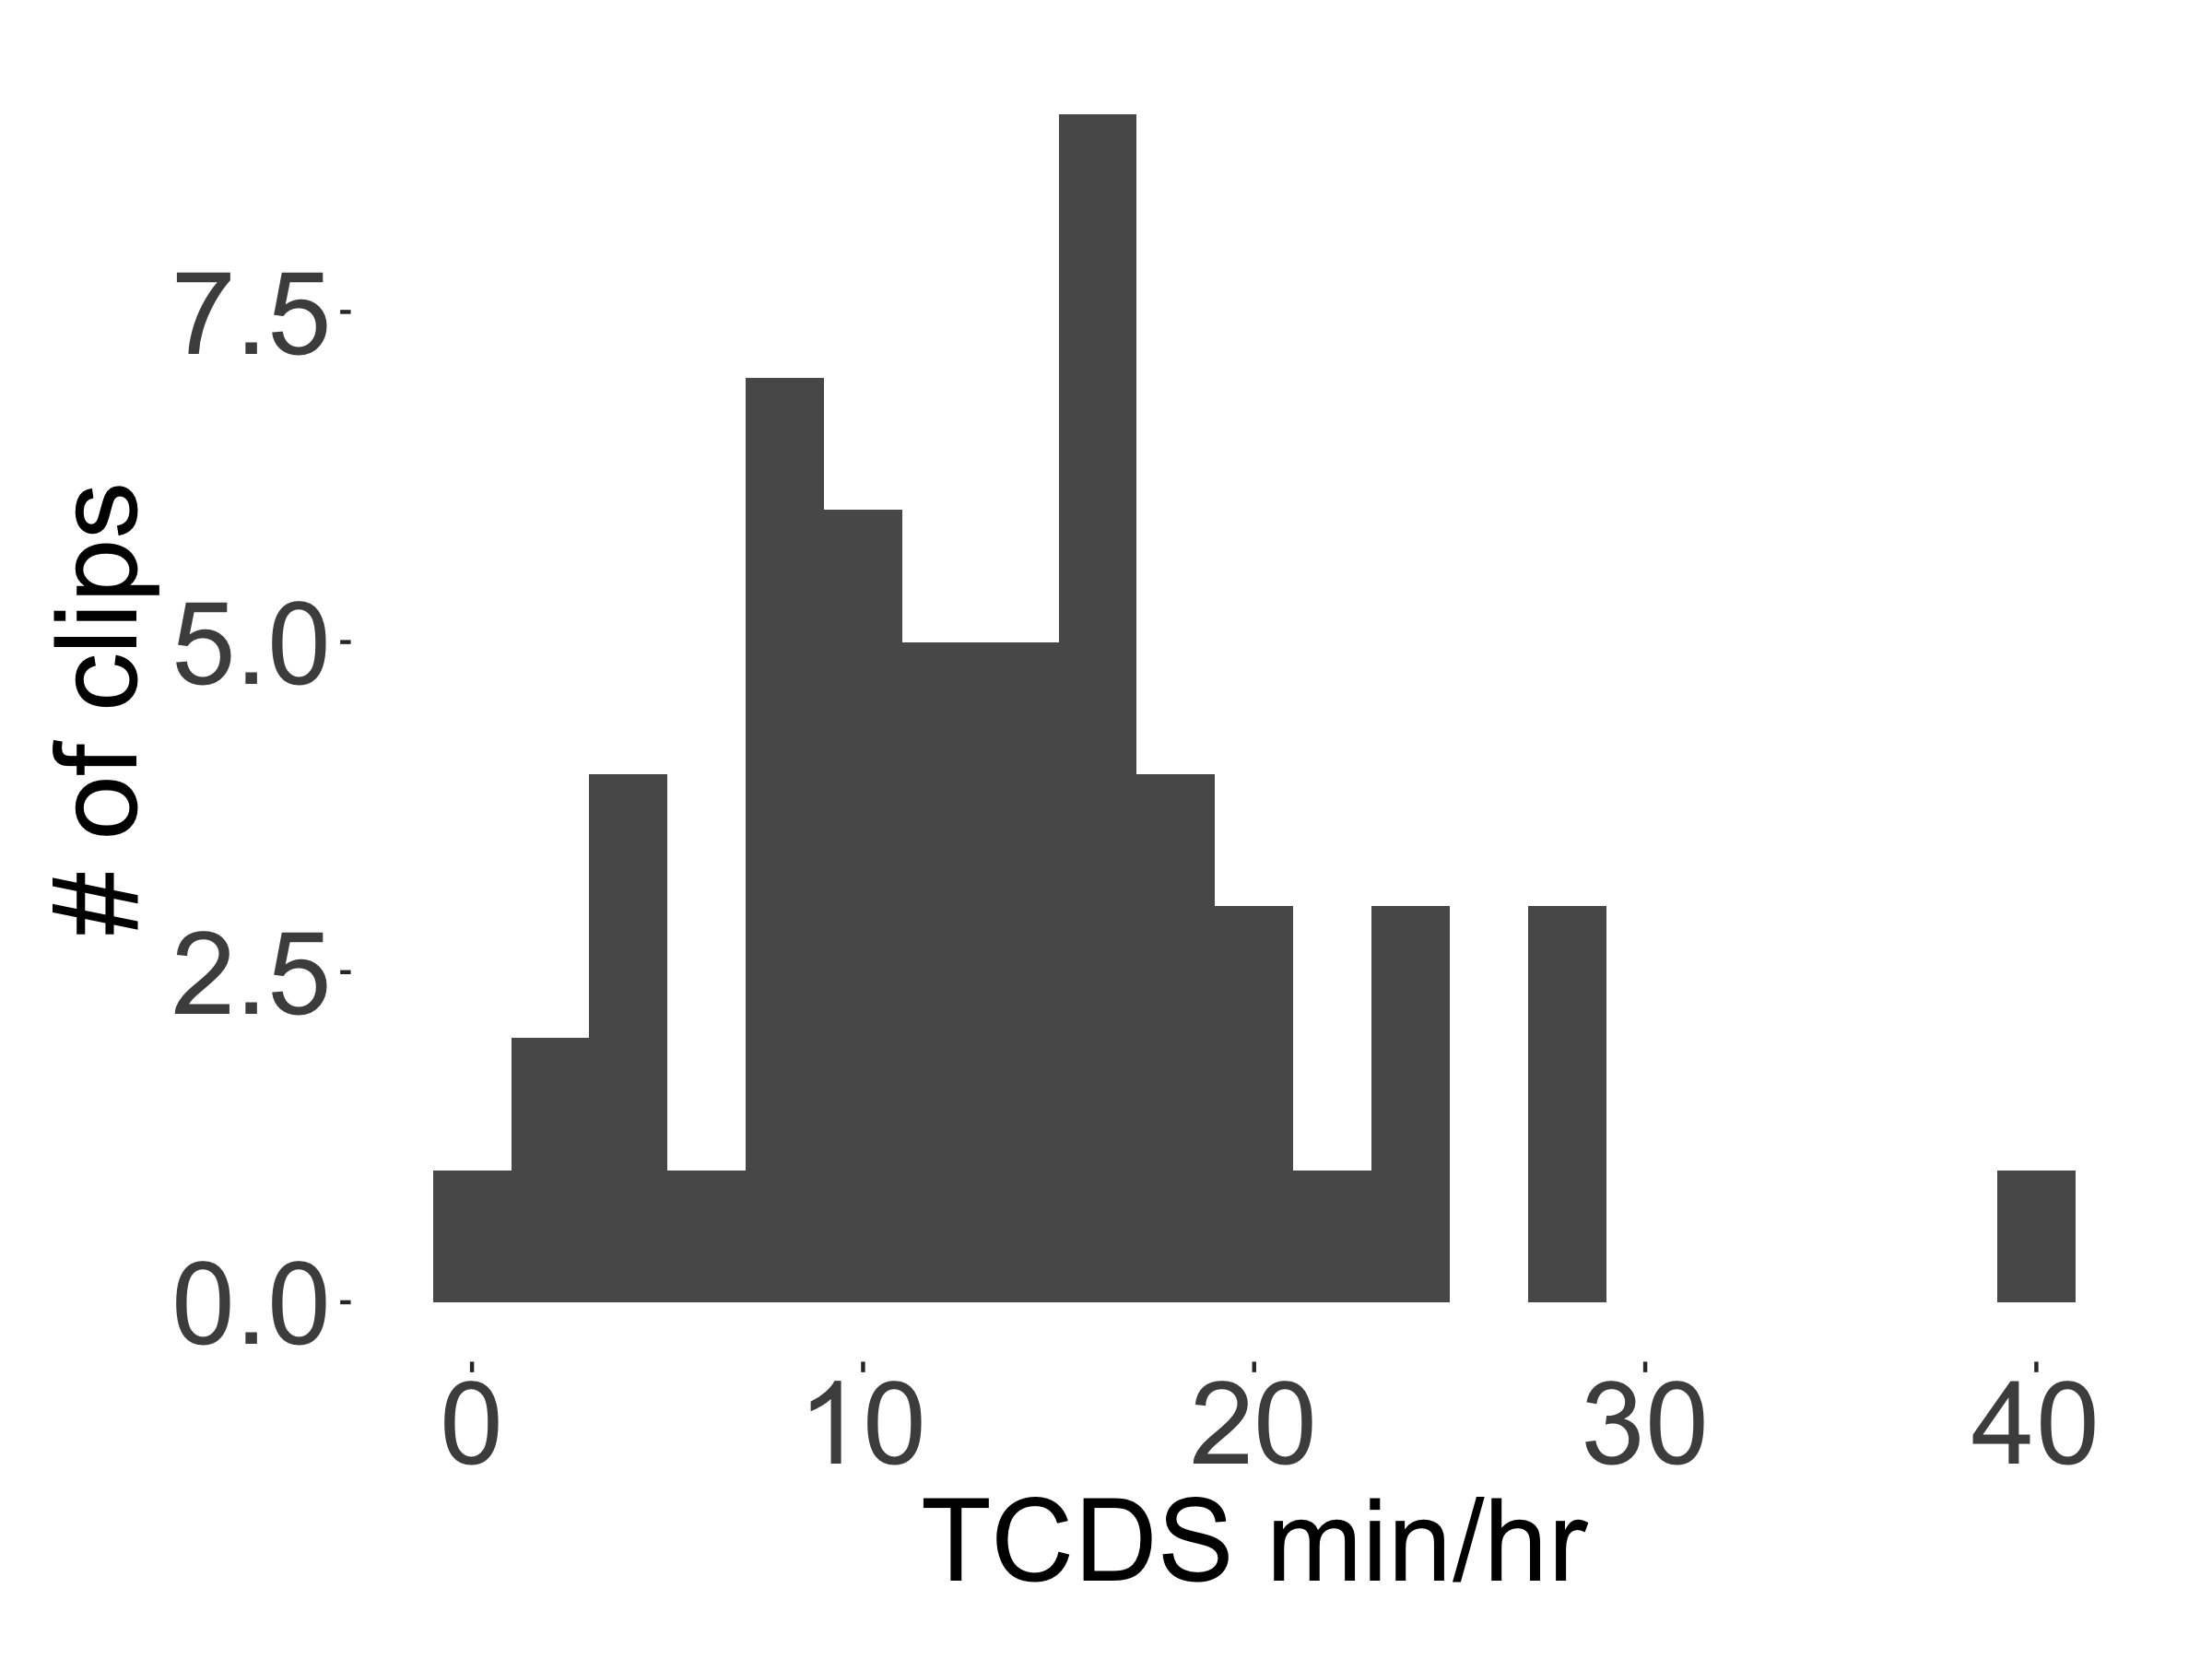
\includegraphics[width=0.4\linewidth]{www/TCDS_turntaking_distribution} 

}

\caption{The distribution of TCDS rates found across the 55 turn-taking clips.}\label{fig:fig4}
\end{figure}

\FloatBarrier

\begin{table}[tbp]
\begin{center}
\begin{threeparttable}
\caption{\label{tab:tab5}Full output of the negative binomial mixed-effects regression of TCDS min/hr for the turn-taking sample, with midday as the reference level for time of day.}
\begin{tabular}{llllll}
\toprule
component & \multicolumn{1}{c}{term} & \multicolumn{1}{c}{estimate} & \multicolumn{1}{c}{std.error} & \multicolumn{1}{c}{statistic} & \multicolumn{1}{c}{p.value}\\
\midrule
cond & (Intercept) & 2.39 & 0.25 & 9.45 & 0.00\\
cond & tchiyr.std & -0.63 & 0.27 & -2.33 & 0.02\\
cond & stthr.trimorning & 0.22 & 0.28 & 0.77 & 0.44\\
cond & stthr.triafternoon & 0.34 & 0.27 & 1.24 & 0.22\\
cond & hsz.std & -0.02 & 0.08 & -0.26 & 0.79\\
cond & nsk.std & -0.04 & 0.09 & -0.52 & 0.60\\
cond & tchiyr.std:stthr.trimorning & 0.53 & 0.28 & 1.89 & 0.06\\
cond & tchiyr.std:stthr.triafternoon & 0.60 & 0.28 & 2.17 & 0.03\\
cond & tchiyr.std:nsk.std & -0.15 & 0.11 & -1.35 & 0.18\\
random\_effect & aclew\_child\_id & 0.00 & NA & NA & NA\\
\bottomrule
\end{tabular}
\end{threeparttable}
\end{center}
\end{table}

\begin{table}[tbp]
\begin{center}
\begin{threeparttable}
\caption{\label{tab:tab6}Full output of the negative binomial mixed-effects regression of TCDS min/hr for the turn-taking sample, with afternoon as the reference level for time of day.}
\begin{tabular}{llllll}
\toprule
component & \multicolumn{1}{c}{term} & \multicolumn{1}{c}{estimate} & \multicolumn{1}{c}{std.error} & \multicolumn{1}{c}{statistic} & \multicolumn{1}{c}{p.value}\\
\midrule
cond & (Intercept) & 2.73 & 0.11 & 23.84 & 0.00\\
cond & tchiyr.std & -0.02 & 0.13 & -0.18 & 0.86\\
cond & stthr.tri.amidday & -0.34 & 0.27 & -1.24 & 0.22\\
cond & stthr.tri.amorning & -0.12 & 0.17 & -0.69 & 0.49\\
cond & hsz.std & -0.02 & 0.08 & -0.26 & 0.79\\
cond & nsk.std & -0.04 & 0.09 & -0.52 & 0.60\\
cond & tchiyr.std:stthr.tri.amidday & -0.60 & 0.28 & -2.17 & 0.03\\
cond & tchiyr.std:stthr.tri.amorning & -0.07 & 0.17 & -0.42 & 0.68\\
cond & tchiyr.std:nsk.std & -0.15 & 0.11 & -1.35 & 0.18\\
random\_effect & aclew\_child\_id & 0.00 & NA & NA & NA\\
\bottomrule
\end{tabular}
\end{threeparttable}
\end{center}
\end{table}

\FloatBarrier

\begin{figure}[H]

{\centering 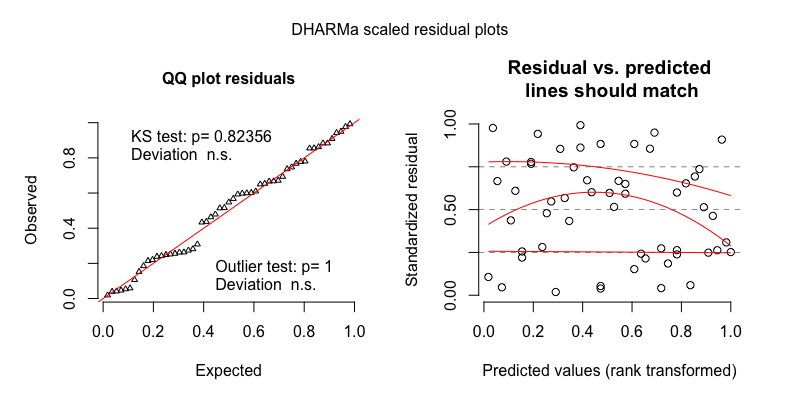
\includegraphics[width=0.9\linewidth]{www/TCDS_turntaking_nb_res_plot} 

}

\caption{The model residuals from the negative binomial mixed-effects regression of TCDS min/hr for the turn-taking sample.}\label{fig:fig5}
\end{figure}

As an alternative analysis we generated parallel models of TCDS rate in
the turn-taking clips using gaussian mixed-effects regression with
logged values of TCDS: results for the two models demonstrating all
pairwise effects of time of day are shown in
\protect\hyperlink{tab7}{Table 7} and \protect\hyperlink{tab8}{Table 8}.
The residuals for the default gaussian model
(\protect\hyperlink{tab7}{Table 7}) are shown in
\protect\hyperlink{fig6}{Figure 6}.

\FloatBarrier

\begin{table}[tbp]
\begin{center}
\begin{threeparttable}
\caption{\label{tab:tab7}Full output of the gaussian mixed-effects regression of TCDS min/hr for the turn-taking sample, with midday as the reference level for time of day.}
\begin{tabular}{llllll}
\toprule
component & \multicolumn{1}{c}{term} & \multicolumn{1}{c}{estimate} & \multicolumn{1}{c}{std.error} & \multicolumn{1}{c}{statistic} & \multicolumn{1}{c}{p.value}\\
\midrule
cond & (Intercept) & 2.32 & 0.24 & 9.69 & 0.00\\
cond & tchiyr.std & -0.84 & 0.24 & -3.44 & 0.00\\
cond & stthr.trimorning & 0.21 & 0.29 & 0.72 & 0.47\\
cond & stthr.triafternoon & 0.36 & 0.26 & 1.36 & 0.18\\
cond & hsz.std & -0.05 & 0.08 & -0.57 & 0.57\\
cond & nsk.std & -0.05 & 0.09 & -0.58 & 0.56\\
cond & tchiyr.std:stthr.trimorning & 0.75 & 0.26 & 2.88 & 0.00\\
cond & tchiyr.std:stthr.triafternoon & 0.81 & 0.26 & 3.14 & 0.00\\
cond & tchiyr.std:nsk.std & -0.18 & 0.12 & -1.48 & 0.14\\
random\_effect & aclew\_child\_id & 0.09 & NA & NA & NA\\
random\_effect & Residual & 0.53 & NA & NA & NA\\
\bottomrule
\end{tabular}
\end{threeparttable}
\end{center}
\end{table}

\begin{table}[tbp]
\begin{center}
\begin{threeparttable}
\caption{\label{tab:tab8}Full output of the gaussian mixed-effects regression of TCDS min/hr for the turn-taking sample, with afternoon as the reference level for time of day.}
\begin{tabular}{llllll}
\toprule
component & \multicolumn{1}{c}{term} & \multicolumn{1}{c}{estimate} & \multicolumn{1}{c}{std.error} & \multicolumn{1}{c}{statistic} & \multicolumn{1}{c}{p.value}\\
\midrule
cond & (Intercept) & 2.68 & 0.13 & 20.54 & 0.00\\
cond & tchiyr.std & -0.03 & 0.16 & -0.19 & 0.85\\
cond & stthr.tri.amidday & -0.36 & 0.26 & -1.36 & 0.18\\
cond & stthr.tri.amorning & -0.15 & 0.21 & -0.73 & 0.47\\
cond & hsz.std & -0.05 & 0.08 & -0.57 & 0.57\\
cond & nsk.std & -0.05 & 0.09 & -0.58 & 0.56\\
cond & tchiyr.std:stthr.tri.amidday & -0.81 & 0.26 & -3.14 & 0.00\\
cond & tchiyr.std:stthr.tri.amorning & -0.07 & 0.20 & -0.33 & 0.74\\
cond & tchiyr.std:nsk.std & -0.18 & 0.12 & -1.48 & 0.14\\
random\_effect & aclew\_child\_id & 0.09 & NA & NA & NA\\
random\_effect & Residual & 0.53 & NA & NA & NA\\
\bottomrule
\end{tabular}
\end{threeparttable}
\end{center}
\end{table}

\FloatBarrier

\begin{figure}[H]

{\centering 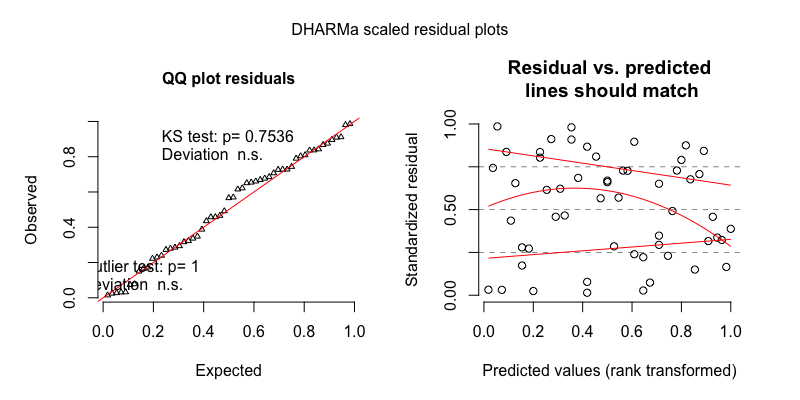
\includegraphics[width=0.9\linewidth]{www/TCDS_turntaking_log_gaus_res_plot} 

}

\caption{The model residuals from the gaussian mixed-effects regression of TCDS min/hr for the turn-taking sample.}\label{fig:fig6}
\end{figure}

\FloatBarrier

\subsection{Other-directed speech (ODS)}\label{models-ods}

\subsubsection{Random clips}\label{models-ods-random}

ODS rate in the random clips demonstrated a skewed distribution, but
without extra cases of zero \protect\hyperlink{fig7}{Figure 7}. We
therefore modeled it using a negative binomial mixed-effects regression
without zero inflation in the main text: results for the two models
demonstrating all pairwise effects of time of day are shown in
\protect\hyperlink{tab9}{Table 9} and \protect\hyperlink{tab10}{Table
10}. The residuals for the default model (\protect\hyperlink{tab9}{Table
9}) are shown in \protect\hyperlink{fig8}{Figure 8}.

\FloatBarrier

\begin{figure}[H]

{\centering 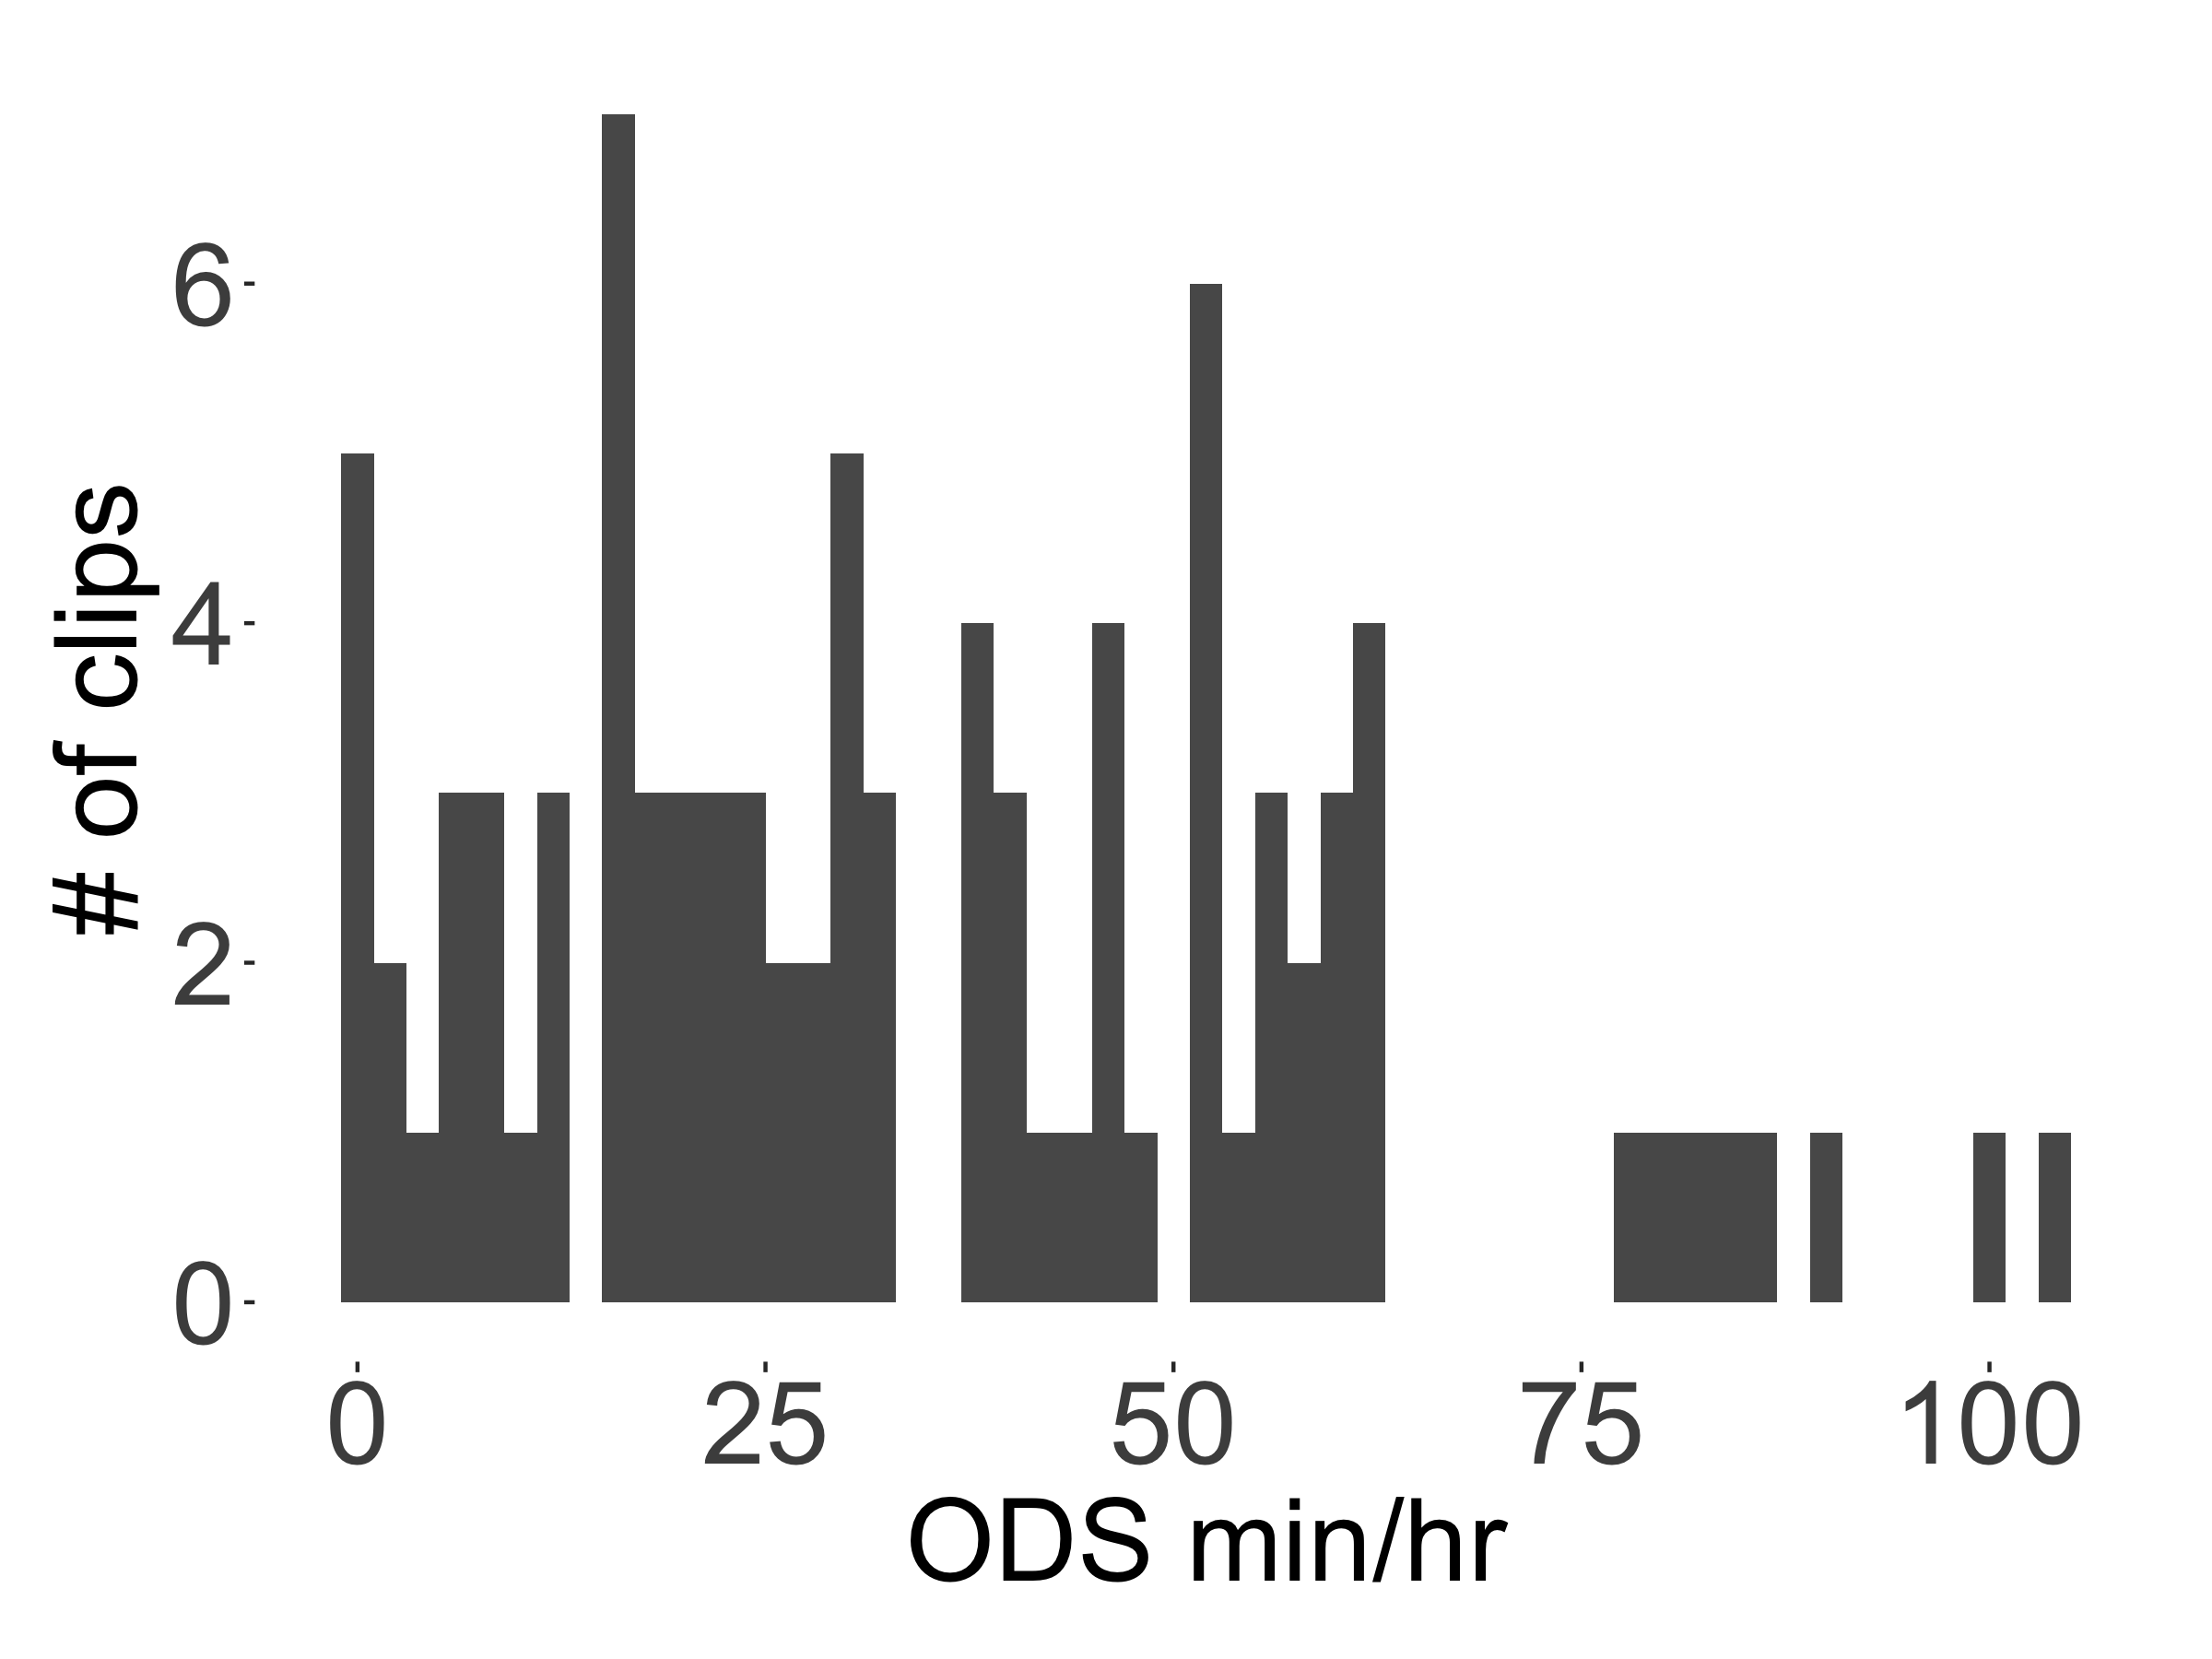
\includegraphics[width=0.4\linewidth]{www/ODS_random_distribution} 

}

\caption{The distribution of ODS rates found across the 90 random clips.}\label{fig:fig7}
\end{figure}

\FloatBarrier

\begin{table}[tbp]
\begin{center}
\begin{threeparttable}
\caption{\label{tab:tab9}Full output of the negative binomial mixed-effects regression of ODS min/hr for the random sample, with midday as the reference level for time of day.}
\begin{tabular}{llllll}
\toprule
component & \multicolumn{1}{c}{term} & \multicolumn{1}{c}{estimate} & \multicolumn{1}{c}{std.error} & \multicolumn{1}{c}{statistic} & \multicolumn{1}{c}{p.value}\\
\midrule
cond & (Intercept) & 3.26 & 0.14 & 23.99 & 0.00\\
cond & tchiyr.std & -0.57 & 0.17 & -3.28 & 0.00\\
cond & stthr.trimorning & 0.20 & 0.16 & 1.19 & 0.23\\
cond & stthr.triafternoon & 0.26 & 0.15 & 1.68 & 0.09\\
cond & hsz.std & -0.02 & 0.06 & -0.32 & 0.75\\
cond & nsk.std & 0.50 & 0.05 & 10.07 & 0.00\\
cond & tchiyr.std:stthr.trimorning & 0.65 & 0.20 & 3.23 & 0.00\\
cond & tchiyr.std:stthr.triafternoon & 0.28 & 0.20 & 1.43 & 0.15\\
cond & tchiyr.std:nsk.std & 0.04 & 0.05 & 0.87 & 0.38\\
random\_effect & aclew\_child\_id & 0.00 & NA & NA & NA\\
\bottomrule
\end{tabular}
\end{threeparttable}
\end{center}
\end{table}

\begin{table}[tbp]
\begin{center}
\begin{threeparttable}
\caption{\label{tab:tab10}Full output of the negative binomial mixed-effects regression of ODS min/hr for the random sample, with afternoon as the reference level for time of day.}
\begin{tabular}{llllll}
\toprule
component & \multicolumn{1}{c}{term} & \multicolumn{1}{c}{estimate} & \multicolumn{1}{c}{std.error} & \multicolumn{1}{c}{statistic} & \multicolumn{1}{c}{p.value}\\
\midrule
cond & (Intercept) & 3.51 & 0.08 & 42.78 & 0.00\\
cond & tchiyr.std & -0.29 & 0.09 & -3.12 & 0.00\\
cond & stthr.tri.amidday & -0.26 & 0.15 & -1.68 & 0.09\\
cond & stthr.tri.amorning & -0.06 & 0.13 & -0.48 & 0.63\\
cond & hsz.std & -0.02 & 0.06 & -0.32 & 0.75\\
cond & nsk.std & 0.50 & 0.05 & 10.07 & 0.00\\
cond & tchiyr.std:stthr.tri.amidday & -0.28 & 0.20 & -1.43 & 0.15\\
cond & tchiyr.std:stthr.tri.amorning & 0.37 & 0.15 & 2.50 & 0.01\\
cond & tchiyr.std:nsk.std & 0.04 & 0.05 & 0.87 & 0.38\\
random\_effect & aclew\_child\_id & 0.00 & NA & NA & NA\\
\bottomrule
\end{tabular}
\end{threeparttable}
\end{center}
\end{table}

\FloatBarrier

\begin{figure}[H]

{\centering 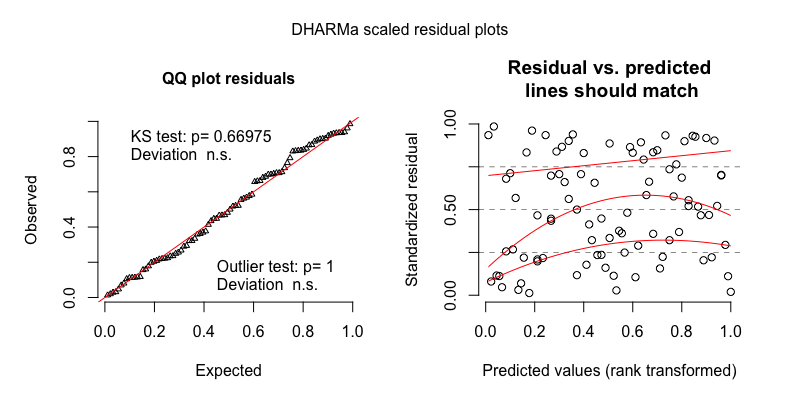
\includegraphics[width=0.9\linewidth]{www/ODS_random_nb_res_plot} 

}

\caption{The model residuals from the zero-inflated negative binomial mixed-effects regression of ODS min/hr for the random sample.}\label{fig:fig8}
\end{figure}

As an alternative analysis we generated parallel models of ODS rate in
the random clips using gaussian mixed-effects regression with logged
values of ODS: results for the two models demonstrating all pairwise
effects of time of day are shown in \protect\hyperlink{tab11}{Table 11}
and \protect\hyperlink{tab12}{Table 12}. The residuals for the default
gaussian model (\protect\hyperlink{tab11}{Table 11}) are shown in
\protect\hyperlink{fig9}{Figure 9}.

\FloatBarrier

\begin{table}[tbp]
\begin{center}
\begin{threeparttable}
\caption{\label{tab:tab11}Full output of the gaussian mixed-effects regression of ODS min/hr for the random sample, with midday as the reference level for time of day.}
\begin{tabular}{llllll}
\toprule
component & \multicolumn{1}{c}{term} & \multicolumn{1}{c}{estimate} & \multicolumn{1}{c}{std.error} & \multicolumn{1}{c}{statistic} & \multicolumn{1}{c}{p.value}\\
\midrule
cond & (Intercept) & 3.06 & 0.16 & 18.79 & 0.00\\
cond & tchiyr.std & -0.48 & 0.16 & -2.98 & 0.00\\
cond & stthr.trimorning & 0.26 & 0.20 & 1.25 & 0.21\\
cond & stthr.triafternoon & 0.28 & 0.18 & 1.55 & 0.12\\
cond & hsz.std & 0.00 & 0.10 & 0.03 & 0.98\\
cond & nsk.std & 0.68 & 0.08 & 8.82 & 0.00\\
cond & tchiyr.std:stthr.trimorning & 0.57 & 0.21 & 2.70 & 0.01\\
cond & tchiyr.std:stthr.triafternoon & 0.09 & 0.18 & 0.51 & 0.61\\
cond & tchiyr.std:nsk.std & 0.04 & 0.07 & 0.63 & 0.53\\
random\_effect & aclew\_child\_id & 0.20 & NA & NA & NA\\
random\_effect & Residual & 0.66 & NA & NA & NA\\
\bottomrule
\end{tabular}
\end{threeparttable}
\end{center}
\end{table}

\begin{table}[tbp]
\begin{center}
\begin{threeparttable}
\caption{\label{tab:tab12}Full output of the gaussian mixed-effects regression of ODS min/hr for the random sample, with afternoon as the reference level for time of day.}
\begin{tabular}{llllll}
\toprule
component & \multicolumn{1}{c}{term} & \multicolumn{1}{c}{estimate} & \multicolumn{1}{c}{std.error} & \multicolumn{1}{c}{statistic} & \multicolumn{1}{c}{p.value}\\
\midrule
cond & (Intercept) & 3.34 & 0.12 & 28.26 & 0.00\\
cond & tchiyr.std & -0.38 & 0.13 & -3.04 & 0.00\\
cond & stthr.tri.amidday & -0.28 & 0.18 & -1.55 & 0.12\\
cond & stthr.tri.amorning & -0.03 & 0.16 & -0.16 & 0.87\\
cond & hsz.std & 0.00 & 0.10 & 0.03 & 0.98\\
cond & nsk.std & 0.68 & 0.08 & 8.82 & 0.00\\
cond & tchiyr.std:stthr.tri.amidday & -0.09 & 0.18 & -0.51 & 0.61\\
cond & tchiyr.std:stthr.tri.amorning & 0.48 & 0.18 & 2.64 & 0.01\\
cond & tchiyr.std:nsk.std & 0.04 & 0.07 & 0.63 & 0.53\\
random\_effect & aclew\_child\_id & 0.20 & NA & NA & NA\\
random\_effect & Residual & 0.66 & NA & NA & NA\\
\bottomrule
\end{tabular}
\end{threeparttable}
\end{center}
\end{table}

\FloatBarrier

\begin{figure}[H]

{\centering 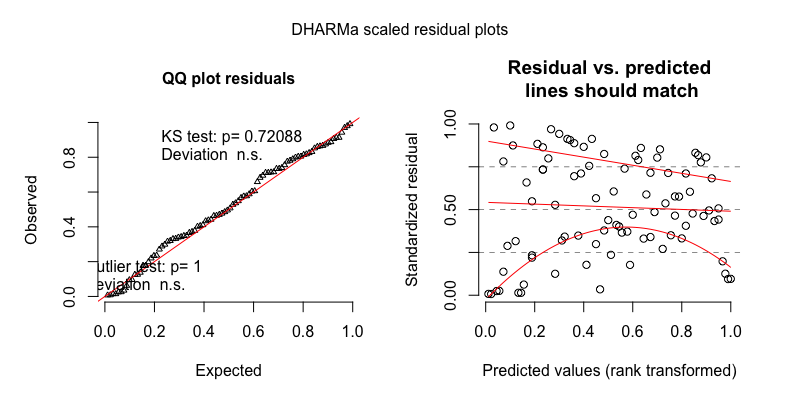
\includegraphics[width=0.9\linewidth]{www/ODS_random_log_gaus_res_plot} 

}

\caption{The model residuals from the gaussian mixed-effects regression of ODS min/hr for the random sample.}\label{fig:fig9}
\end{figure}

\FloatBarrier

\subsubsection{Turn-taking clips}\label{models-ods-turntaking}

ODS rate in the turn-taking clips demonstrated a skewed distribution
\protect\hyperlink{fig10}{Figure 10}. We therefore modeled it using a
negative binomial mixed-effects regression without zero inflation in the
main text: results for the two models demonstrating all pairwise effects
of time of day are shown in \protect\hyperlink{tab13}{Table 13} and
\protect\hyperlink{tab14}{Table 14}. The residuals for the default model
(\protect\hyperlink{tab13}{Table 13}) are shown in
\protect\hyperlink{fig11}{Figure 11}.

\FloatBarrier

\begin{figure}[H]

{\centering 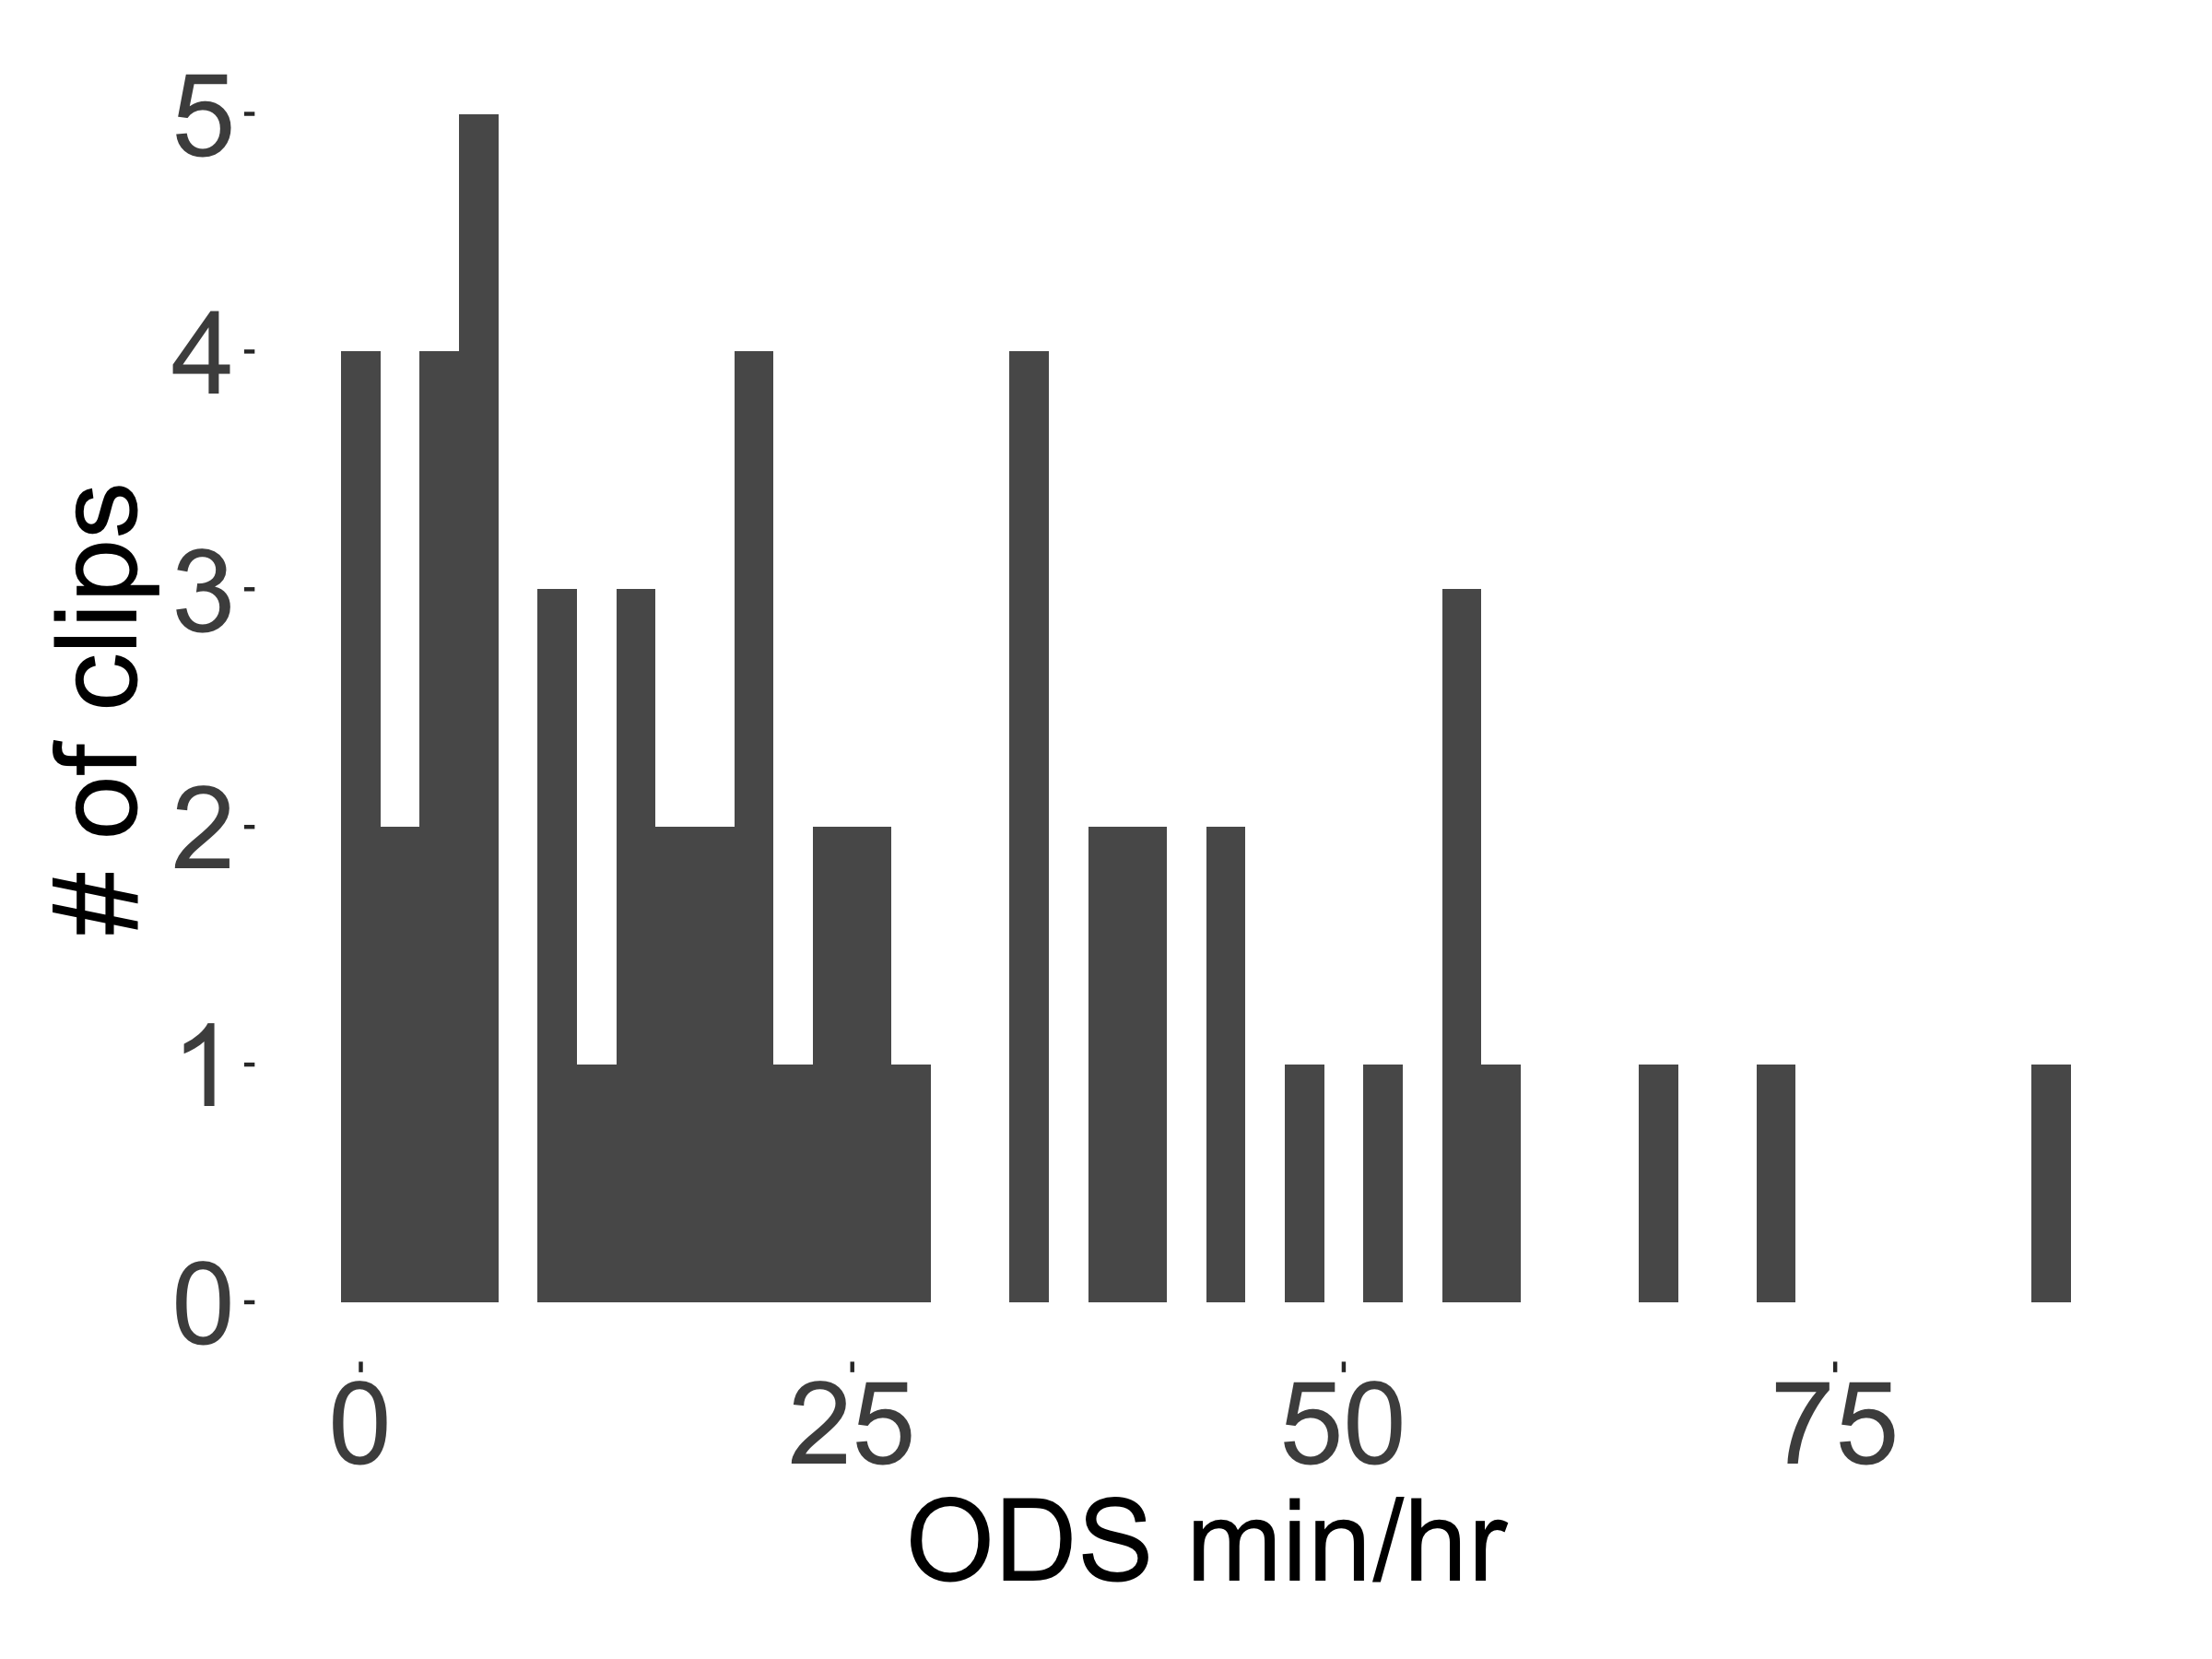
\includegraphics[width=0.4\linewidth]{www/ODS_turntaking_distribution} 

}

\caption{The distribution of ODS rates found across the 55 turn-taking clips.}\label{fig:fig10}
\end{figure}

\FloatBarrier

\begin{table}[tbp]
\begin{center}
\begin{threeparttable}
\caption{\label{tab:tab13}Full output of the negative binomial mixed-effects regression of ODS min/hr for the turn-taking sample, with midday as the reference level for time of day.}
\begin{tabular}{llllll}
\toprule
component & \multicolumn{1}{c}{term} & \multicolumn{1}{c}{estimate} & \multicolumn{1}{c}{std.error} & \multicolumn{1}{c}{statistic} & \multicolumn{1}{c}{p.value}\\
\midrule
cond & (Intercept) & 2.62 & 0.33 & 7.89 & 0.00\\
cond & tchiyr.std & -0.04 & 0.33 & -0.14 & 0.89\\
cond & stthr.trimorning & 0.43 & 0.34 & 1.25 & 0.21\\
cond & stthr.triafternoon & 0.35 & 0.35 & 1.00 & 0.32\\
cond & hsz.std & 0.03 & 0.12 & 0.27 & 0.78\\
cond & nsk.std & 0.56 & 0.08 & 6.76 & 0.00\\
cond & tchiyr.std:stthr.trimorning & -0.15 & 0.33 & -0.44 & 0.66\\
cond & tchiyr.std:stthr.triafternoon & 0.03 & 0.35 & 0.08 & 0.93\\
cond & tchiyr.std:nsk.std & -0.16 & 0.11 & -1.51 & 0.13\\
random\_effect & aclew\_child\_id & 0.28 & NA & NA & NA\\
\bottomrule
\end{tabular}
\end{threeparttable}
\end{center}
\end{table}

\begin{table}[tbp]
\begin{center}
\begin{threeparttable}
\caption{\label{tab:tab14}Full output of the negative binomial mixed-effects regression of ODS min/hr for the turn-taking sample, with afternoon as the reference level for time of day.}
\begin{tabular}{llllll}
\toprule
component & \multicolumn{1}{c}{term} & \multicolumn{1}{c}{estimate} & \multicolumn{1}{c}{std.error} & \multicolumn{1}{c}{statistic} & \multicolumn{1}{c}{p.value}\\
\midrule
cond & (Intercept) & 2.96 & 0.16 & 18.58 & 0.00\\
cond & tchiyr.std & -0.02 & 0.18 & -0.08 & 0.93\\
cond & stthr.tri.amidday & -0.35 & 0.35 & -1.00 & 0.32\\
cond & stthr.tri.amorning & 0.08 & 0.17 & 0.47 & 0.64\\
cond & hsz.std & 0.03 & 0.12 & 0.27 & 0.78\\
cond & nsk.std & 0.56 & 0.08 & 6.76 & 0.00\\
cond & tchiyr.std:stthr.tri.amidday & -0.03 & 0.35 & -0.08 & 0.93\\
cond & tchiyr.std:stthr.tri.amorning & -0.18 & 0.20 & -0.86 & 0.39\\
cond & tchiyr.std:nsk.std & -0.16 & 0.11 & -1.51 & 0.13\\
random\_effect & aclew\_child\_id & 0.28 & NA & NA & NA\\
\bottomrule
\end{tabular}
\end{threeparttable}
\end{center}
\end{table}

\FloatBarrier

\begin{figure}[H]

{\centering 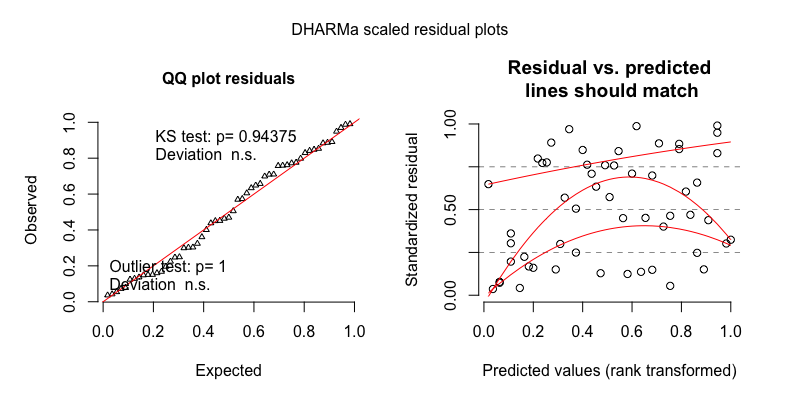
\includegraphics[width=0.9\linewidth]{www/ODS_turntaking_nb_res_plot} 

}

\caption{The model residuals from the negative binomial mixed-effects regression of ODS min/hr for the turn-taking sample.}\label{fig:fig11}
\end{figure}

As an alternative analysis we generated parallel models of ODS rate in
the turn-taking clips using gaussian mixed-effects regression with
logged values of ODS: results for the two models demonstrating all
pairwise effects of time of day are shown in
\protect\hyperlink{tab15}{Table 15} and \protect\hyperlink{tab16}{Table
16}. The residuals for the default gaussian model
(\protect\hyperlink{tab15}{Table 15}) are shown in
\protect\hyperlink{fig12}{Figure 12}.

\FloatBarrier

\begin{table}[tbp]
\begin{center}
\begin{threeparttable}
\caption{\label{tab:tab15}Full output of the gaussian mixed-effects regression of ODS min/hr for the turn-taking sample, with midday as the reference level for time of day.}
\begin{tabular}{llllll}
\toprule
component & \multicolumn{1}{c}{term} & \multicolumn{1}{c}{estimate} & \multicolumn{1}{c}{std.error} & \multicolumn{1}{c}{statistic} & \multicolumn{1}{c}{p.value}\\
\midrule
cond & (Intercept) & 2.55 & 0.29 & 8.92 & 0.00\\
cond & tchiyr.std & -0.12 & 0.30 & -0.40 & 0.69\\
cond & stthr.trimorning & 0.37 & 0.32 & 1.16 & 0.25\\
cond & stthr.triafternoon & 0.31 & 0.30 & 1.02 & 0.31\\
cond & hsz.std & 0.04 & 0.13 & 0.35 & 0.72\\
cond & nsk.std & 0.75 & 0.11 & 6.73 & 0.00\\
cond & tchiyr.std:stthr.trimorning & -0.07 & 0.30 & -0.24 & 0.81\\
cond & tchiyr.std:stthr.triafternoon & 0.21 & 0.30 & 0.70 & 0.48\\
cond & tchiyr.std:nsk.std & -0.20 & 0.14 & -1.37 & 0.17\\
random\_effect & aclew\_child\_id & 0.26 & NA & NA & NA\\
random\_effect & Residual & 0.61 & NA & NA & NA\\
\bottomrule
\end{tabular}
\end{threeparttable}
\end{center}
\end{table}

\begin{table}[tbp]
\begin{center}
\begin{threeparttable}
\caption{\label{tab:tab16}Full output of the gaussian mixed-effects regression of ODS min/hr for the turn-taking sample, with afternoon as the reference level for time of day.}
\begin{tabular}{llllll}
\toprule
component & \multicolumn{1}{c}{term} & \multicolumn{1}{c}{estimate} & \multicolumn{1}{c}{std.error} & \multicolumn{1}{c}{statistic} & \multicolumn{1}{c}{p.value}\\
\midrule
cond & (Intercept) & 2.87 & 0.17 & 17.12 & 0.00\\
cond & tchiyr.std & 0.09 & 0.20 & 0.45 & 0.65\\
cond & stthr.tri.amidday & -0.31 & 0.30 & -1.02 & 0.31\\
cond & stthr.tri.amorning & 0.06 & 0.22 & 0.28 & 0.78\\
cond & hsz.std & 0.04 & 0.13 & 0.35 & 0.72\\
cond & nsk.std & 0.75 & 0.11 & 6.73 & 0.00\\
cond & tchiyr.std:stthr.tri.amidday & -0.21 & 0.30 & -0.70 & 0.48\\
cond & tchiyr.std:stthr.tri.amorning & -0.28 & 0.22 & -1.25 & 0.21\\
cond & tchiyr.std:nsk.std & -0.20 & 0.14 & -1.37 & 0.17\\
random\_effect & aclew\_child\_id & 0.26 & NA & NA & NA\\
random\_effect & Residual & 0.61 & NA & NA & NA\\
\bottomrule
\end{tabular}
\end{threeparttable}
\end{center}
\end{table}

\FloatBarrier

\begin{figure}[H]

{\centering 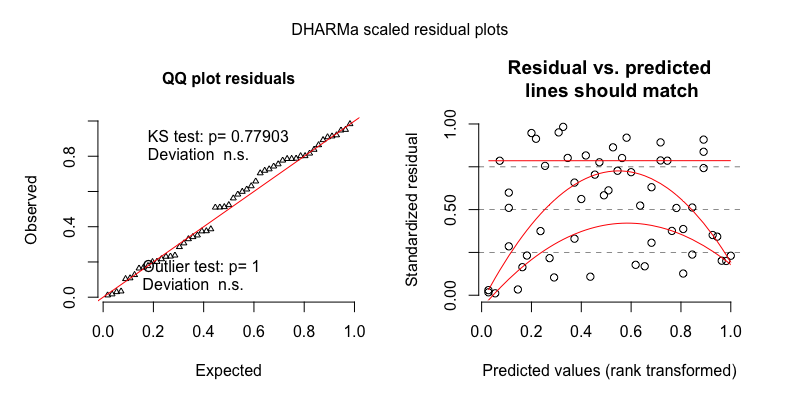
\includegraphics[width=0.9\linewidth]{www/ODS_turntaking_log_gaus_res_plot} 

}

\caption{The model residuals from the gaussian mixed-effects regression of ODS min/hr for the turn-taking sample.}\label{fig:fig12}
\end{figure}

\FloatBarrier

\section{References}\label{refs}

\begingroup
\setlength{\parindent}{-0.5in} \setlength{\leftskip}{0.5in}

\hypertarget{refs}{}
\hypertarget{ref-R-glmmTMB}{}
Brooks, M. E., Kristensen, K., van Benthem, K. J., Magnusson, A., Berg,
C. W., Nielsen, A., \ldots{} Bolker, B. M. (2017a). glmmTMB balances
speed and flexibility among packages for zero-inflated generalized
linear mixed modeling. \emph{The R Journal}, \emph{9}, 378--400.

\hypertarget{ref-brooks2017modeling}{}
Brooks, M. E., Kristensen, K., van Benthem, K. J., Magnusson, A., Berg,
C. W., Nielsen, A., \ldots{} Bolker, B. M. (2017b). Modeling
zero-inflated count data with glmmTMB. \emph{bioRxiv}.
\url{https://doi.org/10.1101/132753}

\hypertarget{ref-casillasFCearly}{}
Casillas, M., Brown, P., \& Levinson, S. C. (forthcoming). Early
language experience in a tseltal mayan village. \emph{Child
Development}, \emph{XX}, XX--XX.

\endgroup


\end{document}
